\section{Ergebnisse}

\subsection{Neue MatchTemplate-Funktion}
Meine finale MatchTemplate-Funktion sieht nun so aus:

\begin{lstlisting}[style=JavaScript]
async function MatchTemplates(src, circle){
    let matchType = cv.TM_CCOEFF_NORMED;
    let iterations = 180;
    let angleStep = 360 / iterations;
    let allResults = [];

    for(let i = 0; i < iterations; i++){
        //pause so the browser can update the gui
        await new Promise(r => setTimeout(r, 0));


        let rotatedSrc = new cv.Mat();
        if(i>0){
            //rotate image
            RotateMatrix(src, rotatedSrc, angleStep * i);
        }else{
            rotatedSrc = src.clone();
        }

        let templateSimilarity = [];
        Object.entries(COINS).forEach(([key, value]) => {

            //check if src and template have the same type
            if(rotatedSrc.type() !== COINS[key].edges.type()){
                console.error("Type of src and template are not the same");
                console.error("src: " + GetMatrixType(rotatedSrc));
                console.error("template(edges): " + GetMatrixType(COINS[key].edges));
                return;
            }

            let templateResized = new cv.Mat();
            cv.resize(COINS[key].edges, templateResized, rotatedSrc.size(), 0, 0, cv.INTER_AREA);

            let resultMat = new cv.Mat();
            cv.matchTemplate(rotatedSrc, templateResized, resultMat, matchType);

            //get highest and lowest value
            let minMax = cv.minMaxLoc(resultMat);
            let max = minMax.maxVal;
            let min = minMax.minVal;

            templateSimilarity.push(new Result(key, min, max));

            //console.log("Match value: " + max);

            //free memory
            templateResized.delete();
            resultMat.delete();
        });

        //find lowest and highest value
        let lowest = templateSimilarity.reduce((prev, current) => (prev.min < current.min) ? prev : current);
        let highest = templateSimilarity.reduce((prev, current) => (prev.max > current.max) ? prev : current);
        allResults.push(new Result("Iteration " + i, lowest, highest));

        //draw loading bar
        DrawLoadingBar(guiMat, (i+1) / iterations);
        DrawMemoryUsage(guiMat);
        //ShowMatrix(guiMat, outputCanvas);
        ShowMatrices([guiMat, COINS[lowest.name].edges, src, rotatedSrc],outputCanvas);
    }

    console.log("Results for all iterations:");
    console.dir(allResults);

    //sort results from highest to lowest
    if (matchType === cv.TM_SQDIFF ||
        matchType === cv.TM_SQDIFF_NORMED) {
        //find lowest value
        allResults.sort((a, b) => a.min.min - b.min.min);
        circle.matchValue = allResults[0].min.min;
        circle.bestMatch = allResults[0].min.name;
    }else{
        //find highest value
        allResults.sort((a, b) => b.max.max - a.max.max);
        circle.matchValue = allResults[0].max.max;
        circle.bestMatch = allResults[0].max.name;
    }

    console.log("Best match:");
    console.dir(allResults[0]);

    //set matchValue to 2 decimal places
    circle.matchValue = Math.round(circle.matchValue * 100) / 100;

    DrawCoinValue([circle], guiMat);

    src.delete();
}
\end{lstlisting}

Lasst uns die Funktion im Detail betrachten:

Zunächst wird die Anzahl der Iterationen für die Rotation festgelegt. In meinem Fall sind es 180, was bedeutet, dass das Bild um 2 Grad pro Iteration gedreht wird und somit insgesamt 180 Bilder erstellt und verglichen werden. Da dies einen hohen Rechenaufwand bedeutet, wird vor jeder Iteration mit \texttt{await new Promise(r => setTimeout(r, 0));} eine kurze Pause eingelegt, damit der Browser die GUI aktualisieren kann. Dafür muss die Funktion als \texttt{async} deklariert sein. Die Rotation erfolgt dann über meine vorher erstellte Funktion \texttt{RotateMatrix}, in welcher der Winkel für die Rotation übergeben wird. 

Nachdem eine Matrix mit dem rotierten Bild erstellt wurde, wird diese mit allen Templates verglichen. Dafür wird über alle Templates iteriert und für jedes Template die Funktion \texttt{cv.matchTemplate} aufgerufen. Die Funktion gibt eine Matrix zurück, in der die Übereinstimmungswerte für das Template und das Bild enthalten sind. Diese Matrix wird dann nach dem höchsten und niedrigsten Wert durchsucht und in einem Array gespeichert.

Für die speicherung der Ergebnisse wird ein Array \texttt{allResults} erstellt, welches Objekte der folgenden Klasse enthält:

\begin{lstlisting}[style=JavaScript]
class Result {
    name;
    min;
    max;

    constructor(name, min, max){
        this.name = name;
        this.min = min;
        this.max = max;
    }

}
\end{lstlisting}

Die Eigenschaften \texttt{min} und \texttt{max} enthalten dabei das Template mit der niedrigsten und höchsten Übereinstimmung. Da manche Vergleichsmethoden den niedrigsten Wert als besten Wert zurückgeben und andere den höchsten, werden somit beide Werte gespeichert. Die Eigenschaft \texttt{name} enthält in der inneren Schleife den Namen des Templates, welches die Übereinstimmung erzielt hat. In der äußeren Schleife wird der Name der Iteration gespeichert.

Innerhalb der inneren Schleife wird pro Vorlage ein Objekt dieser Klasse erstellt und in das Array \texttt{templateSimilarity} gespeichert. Dieses Array enthält somit für diesen Winkel alle Übereinstimmungswerte für alle Vorlagen. Nachdem alle Vorlagen für diesen einen Winkel verglichen wurden, wird das Array \texttt{templateSimilarity} nach dem Ergebnis mit dem niedrigsten und höchsten Wert sortiert und in Form eines neuen Ergebnis-Objektes in das Array \texttt{allResults} gespeichert. Danach iteriert die äußere Schleife weiter und das nächste Bild wird rotiert und verglichen.

Zum Schluss enthält das Array \texttt{allResults} ein Objekt für jede Iteration / jeden Winkel, welches die besten und schlechtesten Übereinstimmungswerte enthält. Je nach Vergleichsmethode wird das Array \texttt{allResults} dann nach dem höchsten oder niedrigsten Wert sortiert und der passendste Wert in das Attribut \texttt{circle.matchValue} zusammen mit dem Namen der Vorlage in \texttt{circle.bestMatch} gespeichert.

Nachdem die Vorlage mit der besten Übereinstimmung gefunden wurde, wird die GUI aktualisiert und das Ergebnis angezeigt. Um den Wert der Münze letztendlich anzuzeigen, wird die Funktion \texttt{DrawCoinValue} aufgerufen, welche den Wert der Münze direkt an die Position der Münze in der GUI einzeichnet. Die Funktion \texttt{DrawCoinValue} sieht wie folgt aus:

\begin{lstlisting}[style=JavaScript]
function DrawCoinValue(circles, dist){
    if (circles === undefined || circles.length === 0) {
        return;
    }

    for(let i = 0; i < circles.length; i++){
        //does circle have "bestMatch" property?
        if (circles[i].bestMatch === undefined) {
            //print "?"
            cv.putText(dist, "?", new cv.Point(circles[i].x, circles[i].y), cv.FONT_HERSHEY_SIMPLEX, 0.5, new cv.Scalar(255, 0, 255, 255), 1);
        }else{
            //print bestMatch
            cv.putText(dist, circles[i].bestMatch, new cv.Point(circles[i].x-10, circles[i].y-6), cv.FONT_HERSHEY_SIMPLEX, 0.5, new cv.Scalar(255, 255, 255, 255), 1);
            cv.putText(dist, circles[i].matchValue.toString(), new cv.Point(circles[i].x-10, circles[i].y+6), cv.FONT_HERSHEY_SIMPLEX, 0.5, new cv.Scalar(255, 255, 255, 255), 1);
        }
    }
}
\end{lstlisting}

\subsection{Finale Ergebnisse}
Nun kommt der Moment der Wahrheit. Wie gut funktioniert die Münzerkennung? Um dies zu überprüfen, habe ich eine kleine Testreihe durchgeführt, bei der ich für 3 verschiedene Einstellungen je 5 Bilder aufgenommen habe. Die Einstellungen waren:

\begin{itemize}
    \item \textbf{180 CCOEFF\_NORMED} - 180 Iterationen, Vergleichsmethode CCOEFF\_NORMED
    \item \textbf{180 SQDIFF\_NORMED} - 180 Iterationen, Vergleichsmethode SQDIFF\_NORMED
    \item \textbf{360 CCOEFF\_NORMED} - 360 Iterationen, Vergleichsmethode CCOEFF\_NORMED
\end{itemize}

Nachdem ich für jede Einstellung 5 verschiedene Bilder aufgenommen ung geprüft habe, bei denen alle 8 Münzen in zufälliger Rotation und Position auf einem Tisch lagen, bin ich zu folgendem Ergebnis gekommen:

\begin{itemize}
    \item \textbf{180 CCOEFF\_NORMED} - Durchschnittliche Erfolgsrate: 67,5\%
    \item \textbf{180 SQDIFF\_NORMED} - Durchschnittliche Erfolgsrate: 60,0\%
    \item \textbf{360 CCOEFF\_NORMED} - Durchschnittliche Erfolgsrate: 62,5\%
\end{itemize}

Die Erfolgsrate ist dabei definiert als die Anzahl der Durchläufe, bei denen die Münze korrekt klassifiziert wurde, geteilt durch die Gesamtanzahl der Durchläufe.

Anschließend habe ich für die Einstellungen mit dem besten Ergebnis (180 CCOEFF\_NORMED) eine weitere Testreihe mit 10 Bildern durchgeführt, um etwas aussagekräftigere Werte zu erhalten. Jedes Bild hatte wie in der vorherigen Testreihe wieder alle verfügbaren Euromünzen in einem zufälligen Winkel abgebildet. Die Ergebnisse sind in Abbildung \ref{fig:SuccessRate} dargestellt:

\begin{figure}[ht]
    \centering
    \caption{Erfolgsrate der Münzerkennung}
    \label{fig:SuccessRate}
    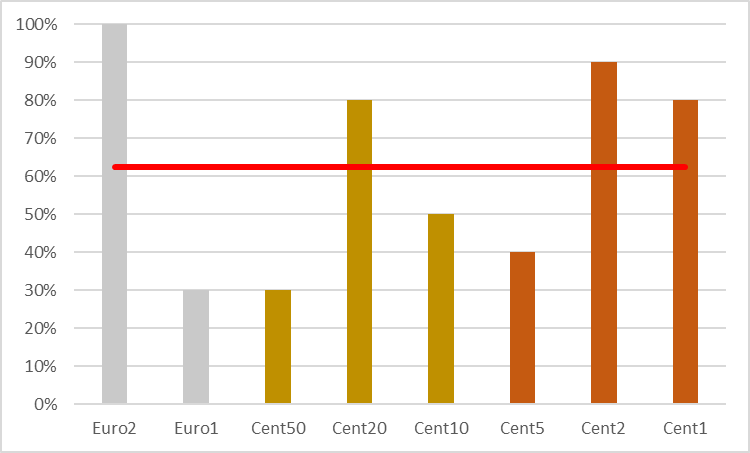
\includegraphics[width=\textwidth]{../SuccessRate2.png}  
\end{figure}

Wie man sofort sieht, gibt es starke Unterschiede in der Erfolgsrate der einzelnen Münzen. Während die 2-Euro Münze in fast allen Fällen korrekt erkannt wurde, lag die Erfolgsquote für die 1 Euro Münze nur bei etwa 30\%. Neben der 2-Euro Münze werden auch die 20-Cent, 2-Cent und 1-Cent Münzen in den meisten Fällen (>50\%) korrekt erkannt. Dagegen werden die 1-Euro, 50-Cent und 5-Cent Münzen nur in etwa 30-40\% der Fälle korrekt erkannt. Für die 10-Cent Münze liegt die Erfolgsrate bei etwa 50\%. Insgesamt beträgt die durchschnittliche Erfolgsrate für alle Münzen somit 62,5\%.

Alles in allem wieder recht durchwachsene Ergebnisse. Zwar konnte ich durch meine Änderungen die Erfolgsrate im Vergleich zu meinem letzten Blogbeitrag auf über 50\% steigern, jedoch ist dies immer noch weit von einer zuverlässigen Münzerkennung entfernt. Die Kantenerkennung scheint dabei der richtige Weg gewesen zu sein, dennoch scheint sie noch nicht einwandfrei zu funktionieren. Die Kanten-Bilder der Vorlagen sehen nahezu perfekt aus, jedoch scheinen besonders die zu prüfenden Münzen nicht immer in ein verwertbares Kantenbild umgewandelt zu werden. Es hat sich als sehr schwierig erwiesen Parameter zu finden, welche für alle Münzen ein gutes Ergebnis liefern, sodass die Konturen der Ziffer klar erkennbar sind, jedoch nicht zu viele Störungen vorhanden sind.

Ich denke jedoch, dass mich dennoch beweisen konnte, dass mittels Template-Matching und OpenCV.js eine Münzerkennung im Browser möglich ist. Die Ergebnisse könnten sicherlich mit etwas weiterem Feintuning verbessert werden, jedoch würde dies den Rahmen dieses Blogs sprengen. Jener Blog neigt sich nun auch dem Ende zu, daher möchte ich im nächsten Abschnitt noch ein Fazit ziehen und einen Ausblick auf mögliche Weiterentwicklungen geben.